% Layout based on Springer Nature's official proceedings samplepaper.tex.
\documentclass[runningheads]{llncs}
\usepackage[T1]{fontenc}
\usepackage{newtxtext}
\usepackage[varvw]{newtxmath}
\usepackage{graphicx,booktabs,array,url}
\usepackage{hyperref}
\let\citep\cite
\let\citet\cite
\providecommand{\tightlist}{\setlength{\itemsep}{0pt}\setlength{\parskip}{0pt}}
\emergencystretch=1.5em
\begin{document}
\title{Cortex AI: Permission-Gated Temporal Retrieval and
Authority-Aware Conflict Abstention for Enterprise Policy Knowledge}
\titlerunning{Permission-Gated Temporal Retrieval for Enterprise Policy}
\author{Aditya Gholap \and Arya Dhumal \and Ashwin Gudur \and Yashraj
Bansal}
\authorrunning{A. Gholap et al.}
\institute{Department of Computer Science and Engineering, MIT School of
Computing, MIT Art, Design and Technology University, Pune,
India\\{[}Corresponding author and email to be confirmed{]}}
\maketitle
\begin{abstract}
Enterprise policy questions require evidence that the requester may
read, that applies on the requested date, and that supports a decision
when sources disagree. Cortex AI integrates tenant-scoped document
grants, reviewed effective intervals and structured claims,
authority-aware conflict abstention, and version-bound citations in an
implemented policy-answering system. A lexical match opens a bounded set
of approved, applicable peers so that the highest-ranked conflicting
claims remain visible to the decision rule. The system emits a templated
answer only when its selected evidence supports it or when a current,
verified Auditor decision resolves the exact conflict. Separate passage
search can use local semantic retrieval without changing the governing
claim. On the original development fixture, the evaluator reproduced 12
of 12 expected outcomes, 15 of 15 labeled authorized peers, and 10 of 10
citation span and hash checks. On a second fictional corpus, the
complete system matched the labeled outcomes and selected sources for
all 16 queries. A recency comparator matched 5, and both valid-time
comparators matched 14 because each committed on two questions about the
same unresolved conflict. The evaluation bounds the evidence to
fictional policies and the checked application stages.
\keywords{enterprise policy retrieval · access control · valid time ·
conflict abstention · evidence provenance}
\end{abstract}
\section{Introduction}\label{introduction}

An employee asking how many days of annual leave apply may find a
current policy, a historical edition, and an approved revision that will
become effective next year. All three can match the same query. The
revision published most recently can be wrong for the requested date.
Two genuinely contradictory sources may also govern at the same time, in
which case an answer backed by only one can conceal a disagreement that
matters to the employee. Access rights add another constraint. Evidence
available to a policy administrator may be inaccessible to the employee
whose question the system answers.

Knowledge-management research documents organizational barriers to
finding and using internal knowledge \citep{alavi}. Retrieval-augmented
generation shows how retrieved documents can ground open-domain answers
\citep{lewis}. Policy answering adds a decision about which sources are
admissible and which claims govern. A genuine citation to a
future-effective edition or to only one of two competing sources can
still support the wrong decision.

Cortex AI implements a bounded evidence decision system. It answers
reviewed numeric policy questions in four topics: annual leave, remote
work, notice period, and executive bonus. Its decision integrates
current tenant and document authorization, reviewed effective dates and
scope, expansion of comparable claims, authority ranking, conflict
abstention, and exact-span verification. It can also expose an
explicitly recorded human resolution of an exact conflict. These are
established ideas from access control, information retrieval and
selective prediction. The contribution is their integration into an
inspectable implementation, with one evaluation protocol following the
final value or abstention back to the authorized evidence set and cited
edition.

We reproduce the development checks and evaluate a second fictional
corpus with new texts and predeclared applicability and disagreement
labels. The drafting workflow constructed and evaluated this corpus.
External adjudication remains open. A separate passage-retrieval
comparison measures a different output from the strict decision.

\section{Related Work}\label{related-work}

\subsection{Enterprise authorization and lexical
retrieval}\label{enterprise-authorization-and-lexical-retrieval}

The NIST role-based access control model formalizes the relationship
among users, roles and permissions \citep{sandhu}. Cortex uses roles for
action permissions and document grants for resource visibility.
B\"{u}ttcher and Clarke studied access-aware full-text search over a
shared filesystem index and showed that simple postprocessing can expose
information about hidden files \citep{buettcher}. Their work motivates a
careful distinction between database index access and the text or
ranking statistics available to an application stage. Cortex's shared
full-text index stays inside its trusted database. Query eligibility
constrains which IDs are returned, and application ranking is computed
on admitted records. The experiments observe application boundaries and
do not establish the filesystem study's broader security properties.

BM25 formalizes probabilistic lexical ranking \citep{robertson}. BEIR
shows the importance of lexical baselines on diverse retrieval tasks
\citep{thakur}. Dense Passage Retrieval shows how learned
representations retrieve passages that need not share surface terms with
the question \citep{karpukhin}. Reciprocal rank fusion combines ranked
lists without requiring scores on a common scale \citep{cormack}. These
works motivate testing lexical and semantic passage recall
independently. They do not prescribe whether a current policy may
override another policy or authorize text retrieval for a given reader.

\subsection{Valid time, contradiction and
support}\label{valid-time-contradiction-and-support}

Time-aware models condition answers on changing facts \citep{dhingra}.
HoH examines coexistence of stale and current information in
retrieval-augmented answering \citep{ouyang}. Re3 uses relevance and
recency with conflict-aware temporal filtering \citep{cao}. TimelyRAG
reranks passages by clause-level validity in evolving documents
\citep{nam}. Cortex takes an effective interval from reviewed metadata
and accepts a requested past, current or future date. Publication
recency is a useful comparator because it implements a different notion
of precedence.

MultiNLI studies entailment, neutrality and contradiction in sentence
pairs \citep{williams}. Ragability evaluates language models given
conflicting and consistent contexts \citep{gross}. Cortex uses a
narrower decision rule: differing normalized integers within the same
policy claim key and strongest authority tier. That restriction allows a
deterministic test of the rule. It also excludes linguistic exceptions,
modality shifts outside the schema and contradictions spread over
several clauses. Selective classification supplies the concepts of risk
and coverage \citep{geifman}. Here, answer coverage can be counted
directly and abstention is triggered by explicit rules, including
missing evidence and unresolved equal-tier disagreement.

ALCE separates citation support from completeness \citep{gao}. RAGAs
separates retrieval and answer quality \citep{es}, and Self-RAG learns
when to retrieve and critique \citep{asai}. Cortex tests substring
equality and the reviewed number before rendering a fixed sentence.
Human review remains responsible for interpretation. Corpus poisoning
research motivates controlling which versions become eligible
\citep{zou}. The effectiveness of review against malicious approved
content remains untested.

\section{Problem Definition and Research
Questions}\label{problem-definition-and-research-questions}

The input to the strict path is a request \(q=(u,t,s,k)\) consisting of
an authenticated user \(u\), an as-of date \(t\), requested scope \(s\)
and a supported policy topic \(k\). Scope includes jurisdiction and
population and assumes the supported default condition. The system maps
a finite policy intent to an expected predicate and unit. Each reviewed
candidate carries a normalized claim value, a source version, a span of
extracted text, applicability metadata and a source authority rank. A
query can return a supported numeric answer, an abstention with a reason
or a request for clarification. A genuine unresolved conflict can carry
several citations even when it returns no governing value.

\textbf{RQ1.} How do reviewed approval, scope and effective-date
filtering affect policy selection compared with lexical candidates
ordered by publication recency? \textbf{RQ2.} When applicable claims
disagree, how often does strongest-tier abstention avoid a conflicting
commitment, and does it retain consistent revisions and equivalent
claims as negative controls? \textbf{RQ3.} In the tested threat model,
does tenant and document authorization prevent restricted text from
entering the application reasoning and output stages? \textbf{RQ4.} Can
a reader use each citation to recover the exact reviewed span of the
identified version and verify the text hash? \textbf{RQ5.} What
additional passage matches and warm request-time cost are observed when
the optional local encoder is enabled?

\section{System Architecture and Trust
Model}\label{system-architecture-and-trust-model}

Figure 1 shows the principal data flows. The browser sends requests to a
FastAPI service. The service derives identity from an opaque session and
checks tenant-local actions before processing protected endpoints. The
authorization predicate for a document requires a same-tenant,
unarchived record and a current direct user or role READ grant. Role
membership determines allowed actions, and administrating a document
workflow does not by itself authorize reading any document in the
tenant.

\begin{figure}
\centering
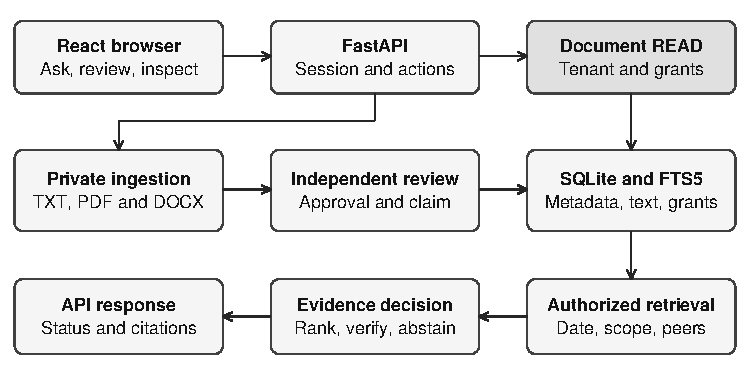
\includegraphics[width=0.89\linewidth,height=\textheight,keepaspectratio,alt={System
architecture. Browser and API actions connect to tenant and document
checks, ingestion, independent review, the evidence store, retrieval,
and answer rendering.}]{../figures/rendered/fig1.pdf}
\caption{System architecture. Browser and API actions connect to tenant
and document checks, ingestion, independent review, the evidence store,
retrieval, and answer rendering.}\label{fig:architecture}
\end{figure}

The three roles are Employee, Auditor and Admin. Employees ask policy
questions and can refer an actual unresolved answer for re-audit. Admin
operates accounts, distribution and policy submission workflows.
Auditors review policies independently and can examine exact conflict
sources when granted access. Approval and distribution are distinct
operations. The application checks current access again when an answer,
source or version is opened. Current permission also governs historical
questions, so moving the answer date into the past does not restore an
earlier document grant.

The threat model covers a requester with limited permissions, a separate
tenant, stale access after revocation, and stored-data changes
detectable by the checks. The process, configured signing key and
database are trusted. Compromised servers, reviewers who collude,
shared-resource timing, and previously disclosed copies are outside the
model. A process lock and transaction bound consistency to the supported
single-process configuration.

\section{Methodology}\label{methodology}

\subsection{Admission and peer
expansion}\label{admission-and-peer-expansion}

For a clause \(c\), let \(G(u,c)\) indicate the tenant and READ check,
\(A(c)\) approved current metadata with an active authority rule, and
\(S(c,q)\) the strict topic, population, jurisdiction, subject, modality
and condition predicates. Let \(b_c\) be the effective start and \(e_c\)
be the effective end, with a missing end interpreted as open. An
eligible clause satisfies

\[G(u,c)\land A(c)\land S(c,q)\land b_c\leq t\land(t<e_c\ \lor\ e_c=\varnothing).\]

One SQL statement combines reviewed eligibility with a full-text match
and returns only clause IDs. The logical candidate boundary is
independent of the database's physical execution order. A bounded token
and synonym expression must match at least one eligible ID. The service
then loads all admitted peers within the cap, checks the expected
predicate and unit, and sorts authorized text by token occurrence with
an identifier tie-break. Even a peer with lower lexical overlap can
participate in the decision. Figure 2 traces the stages.

\begin{figure}
\centering
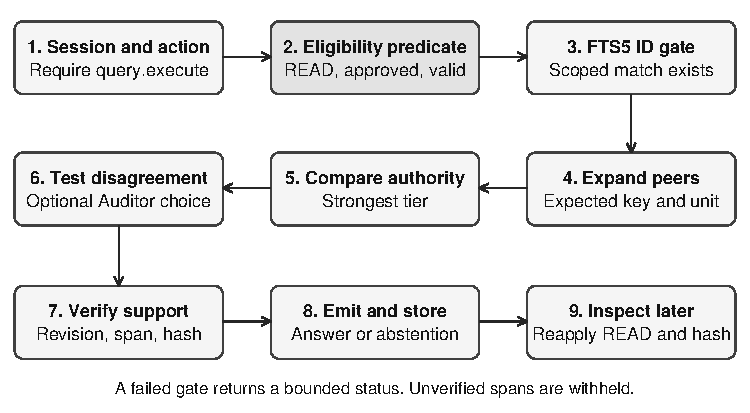
\includegraphics[width=0.89\linewidth,height=\textheight,keepaspectratio,alt={Strict
policy pipeline. The API combines authorization and reviewed eligibility
with the FTS identifier gate, expands peers, compares authority and
verifies evidence before returning a
status.}]{../figures/rendered/fig2.pdf}
\caption{Strict policy pipeline. The API combines authorization and
reviewed eligibility with the FTS identifier gate, expands peers,
compares authority and verifies evidence before returning a
status.}\label{fig:pipeline}
\end{figure}

Time validity is half-open. If one edition ends when its successor
begins, exactly one is eligible on the transition date, provided the
other predicates hold. Figure 3 illustrates a leave revision already
issued on the question date but not yet applicable. The strict
implementation stores publication and ingestion information separately
and does not use them as eligibility cutoffs. An applicable clause is
therefore not evidence about what was physically available to a past
reader. A bitemporal reconstruction would additionally need a
transaction-time history and was outside the current method.

\begin{figure}
\centering
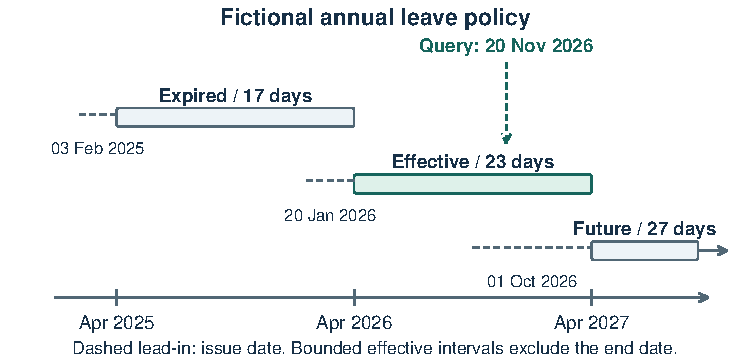
\includegraphics[width=0.89\linewidth,height=\textheight,keepaspectratio,alt={Fictional
leave policy timeline. On 20 November 2026 the April 2026 edition
applies although a future-effective edition has already been
issued.}]{../figures/rendered/fig3.pdf}
\caption{Fictional leave policy timeline. On 20 November 2026 the April
2026 edition applies although a future-effective edition has already
been issued.}\label{fig:timeline}
\end{figure}

\subsection{Authority, disagreement, and human
resolution}\label{authority-disagreement-and-human-resolution}

A strict comparison requires the topic's governing source kind to be
present: an operations policy for remote work or an HR policy for the
other three topics. The service checks that comparable claims share a
single key, then considers the highest rank among the admitted peers. If
those strongest claims have one value, the system can cite up to eight
supporting spans. If there are different values in the highest tier, it
normally abstains and cites the disagreement. A strongest tier with too
many conflicting spans or a candidate pool beyond the peer bound
produces an evidence-limit abstention. Lower-tier differences cannot
force a conflict under this rule. Figure 4 illustrates how interval
filtering removes a replaced edition before the disagreement test, and
why actual concurrent claims can remain incompatible.

\begin{figure}
\centering
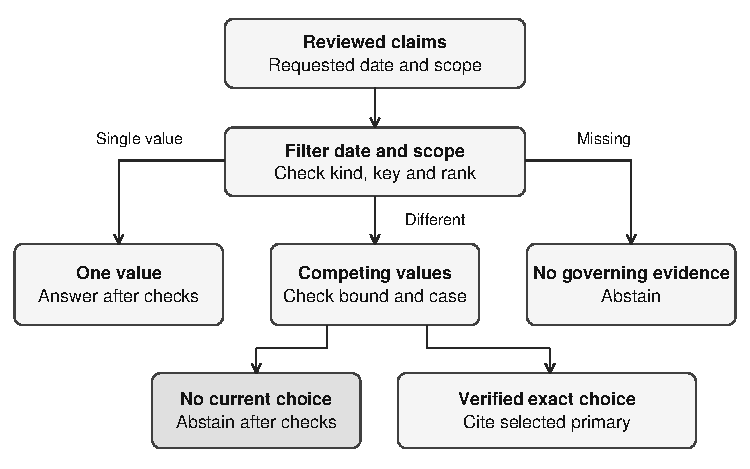
\includegraphics[width=0.89\linewidth,height=\textheight,keepaspectratio,alt={Authority
and conflict decision. Current competing values at the strongest tier
cause abstention unless an exact currently verified Auditor choice
applies.}]{../figures/rendered/fig4.pdf}
\caption{Authority and conflict decision. Current competing values at
the strongest tier cause abstention unless an exact currently verified
Auditor choice applies.}\label{fig:authority}
\end{figure}

The re-audit workflow starts from an owned, still-actionable conflict
query. The server recomputes the authorized conflict and derives a
fingerprint from the sorted evidence, including identifiers, claim keys,
authority ranks, validity windows, values and hashes. An Auditor can
choose a primary from the exact version set after checks. If a later
request maps to that same current conflict, the primary can supply an
answer after integrity checks, with the human choice identified. Undo
removes the choice and restores baseline abstention. A new claim,
changed authority, changed visible peer set or withdrawn READ can make
the previous choice inapplicable. The workflow adds explicit audited
source grants for the Auditor when a qualifying case requires them. It
does not add READ for the Employee.

\subsection{Citation verification and
provenance}\label{citation-verification-and-provenance}

For an evidence record with extracted text \(T\), offsets \(i,j\) and
stored digest \(h\), fresh strict support checks require \(T[i:j]\) to
equal the quoted text and \(\mathrm{SHA256}(\mathrm{UTF8}(T))=h\). The
comparison also checks that the reviewed integer appears as a whole
numeric match. The query response includes exact version and clause IDs,
passage locators and offsets. The saved-answer path checks owner,
retention, current READ and dependency revisions, and verifies the
extracted-text digest. A grant or knowledge revision can invalidate a
saved result conservatively even when a particular cited passage was
unaffected. Figure 5 connects the evidence entities used in these
checks.

\begin{figure}
\centering
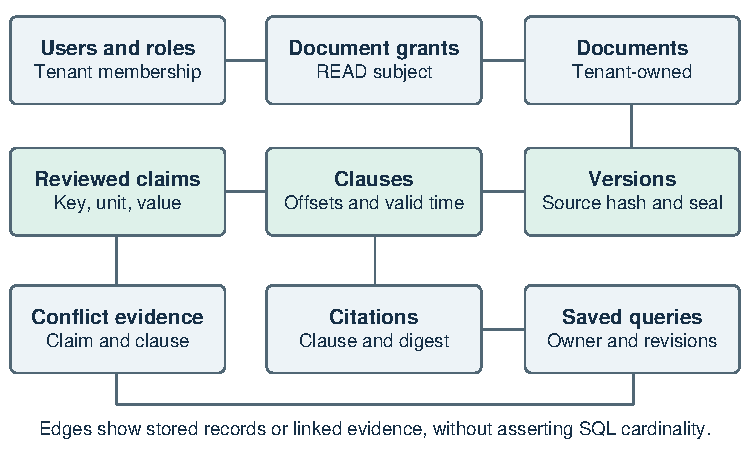
\includegraphics[width=0.89\linewidth,height=\textheight,keepaspectratio,alt={Evidence
relationships. User and role grants connect to documents and versions,
with approved clauses giving rise to claims, citations and conflict
evidence.}]{../figures/rendered/fig5.pdf}
\caption{Evidence relationships. User and role grants connect to
documents and versions, with approved clauses giving rise to claims,
citations and conflict evidence.}\label{fig:evidence}
\end{figure}

The system also stores an Ed25519 signature over a canonical upload
manifest \citep{rfc8032}. The manifest binds the tenant and version
identity to original-byte and extracted-text hashes and supplied
provenance fields. The integrity endpoint checks the configured key
identity, signature, stored metadata and independent hashes of the file
and extracted text. Re-audit resolution and reuse additionally check
signed source integrity. Ordinary strict answers rely on span, numeric
occurrence and extracted-text digest checks, so a routine citation
should not be interpreted as a fresh signature verification. A valid
seal establishes correspondence with the locally configured signer and
stored data. It cannot certify that a policy was authorized by an
external institution or that its content is correct.

\section{Implementation}\label{implementation}

We evaluated GitHub main commit
\href{https://github.com/NoirPrimordial7/cortex-ai/commit/dbbd2f293f312f3055db6beffc045e3e5b7ee62a}{dbbd2f2}.
React presents the question, date, scope and sources. FastAPI and
SQLAlchemy implement the protected boundary and tenant-qualified queries
against SQLite and FTS5. Alembic versions the schema. A bounded child
process extracts TXT, PDF and DOCX and retains original bytes privately.
A reviewer selects a span and numeric claim. The parser runs under the
local account, and pending versions remain outside retrieval.

The broader related-passage path has a different contract. It selects
eligible lexical candidates, computes BM25 on those candidates and can
add cosine-ranked vectors from the pinned local MiniLM encoder.
Reciprocal rank fusion combines the two rankings with a reciprocal
offset of 60. This path can surface passages for queries without a
strict policy answer. It rechecks each selected passage against its
extracted-text digest and offsets. Semantic ranking does not change the
strict peer set or substitute a passage for a reviewed claim. The
application also supports personal leave records under separate
authorization. The evaluation deliberately excludes that transactional
path.

\section{Experimental Setup}\label{experimental-setup}

Figure 6 describes the two evaluation strata. The existing evaluator
seeds the development database and executes the repository's 12 cases.
Labels include status, selected clause IDs and eligible peer IDs.
Instrumentation observes admitted evidence in reasoning, selected
evidence in the answerer and a restricted marker in the response. The
evaluator opens the citation endpoint and recomputes the text hash. The
case count is distinct from frontend unit regressions, backend
regressions and actual browser flows.

\begin{figure}
\centering
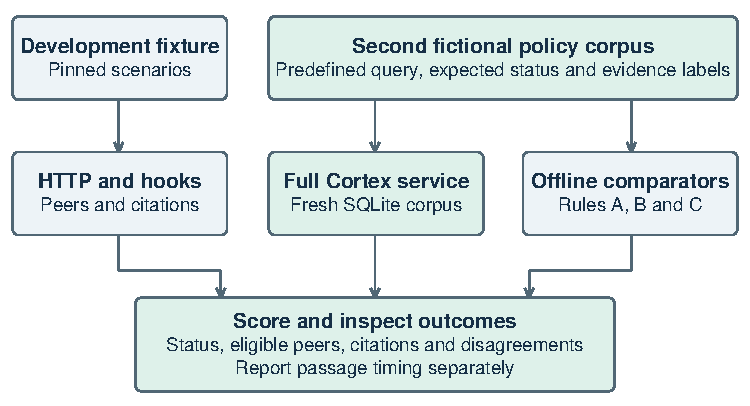
\includegraphics[width=0.89\linewidth,height=\textheight,keepaspectratio,alt={Evaluation
workflow. The development fixture and new fictional benchmark exercise
the pinned service, and offline comparator rules operate on the same
visible fictional policies.}]{../figures/rendered/fig6.pdf}
\caption{Evaluation workflow. The development fixture and new fictional
benchmark exercise the pinned service, and offline comparator rules
operate on the same visible fictional policies.}\label{fig:evaluation}
\end{figure}

The new fixture contains 12 short fictional policies and 16
date-and-scope questions. We define the policy's expected value or
abstention reason, all admitted peers, and selected citation set before
executing the service. The script seeds identities and roles in an
isolated database, removes employee visibility of original seed
documents there, and submits new policy text through the real ingestion,
approval and distribution routes. The new corpus includes one pending
document and one approved document without Employee READ. Numeric
values, windows and labels are in the reproducibility package. The
historical remote edition, the exact expiry of a competing edition, and
concurrent policies with equal values are negative controls for conflict
detection. Two questions ask during the same conflicting pair's overlap.
They are two observations of one underlying conflict.

The decision comparators share approved, visible sources, topic and
population. A selects the most recently published source among lexical
matches and ignores effective intervals and authority. B imposes valid
time and selects a BM25 match without authority or conflict abstention.
C restricts B to the governing source kind, which represents the
strongest tier in this specific fictional corpus, then commits to the
leading match even when its peers disagree. D is the intact service. A
through C execute offline against the labeled corpus, while D executes
through the real HTTP boundary. This supports a comparison of selected
outcomes under declared rules. It does not isolate individual causal
effects on production latency.

We measure recovery and exact identities of eligible peers and selected
evidence. Conflict precision and recall use predicted and labeled
conflicts respectively, and the false-positive rate uses labeled
negatives. Coverage is the proportion receiving a value. Citation checks
re-fetch the exact version and recompute its digest. Exposure checks use
canaries in observed stages and payloads plus specific denied reads.
In-process warm requests include SQLite persistence and TestClient
overhead. The host ran Windows 11 with an Intel Core i7-13700F, Python
3.12.10, SQLite 3.49.1, FastAPI 0.143.0 and SQLAlchemy 2.0.54. The
strict warm workload uses one annual-leave prompt, five preliminary
requests and 50 measured calls, with the optional related-passage model
configured.

\section{Results}\label{results}

\subsection{Development fixture and software
verification}\label{development-fixture-and-software-verification}

The original fixture reproduced 12/12 expected outcomes, 15/15 labeled
authorized peers and 10/10 exact-span and hash checks. All five temporal
cases and all four expected abstentions passed. One conflict query was
labeled positive and correctly detected, with zero false positives or
misses in that fixture. The checked restricted marker did not occur in
reasoning, selected evidence or response payloads. These are designed
regression scenarios rather than an estimate of expected production
accuracy. The earlier governance report records 97 backend tests, 39
frontend tests and 13 real-browser scenarios. The pinned main report
records an expanded suite after conflict-driven re-audit. Our rerun
passed 107 backend tests, including real MiniLM inference, 44 frontend
tests, and all six real Chrome scenarios for the conflict re-audit flow
and responsive widths. The backend run emitted one TestClient
deprecation warning. These counts describe software regression checks
rather than independent observations of policy correctness.

\subsection{New fictional policies and decision
rules}\label{new-fictional-policies-and-decision-rules}

The complete service matched status, reason, value and selected sources
on 16/16 questions and retrieved all 19 eligible policy-question pairs
with no extra peers. It detected both conflict queries (2/2 precision
and 2/2 recall), with zero false conflicts among 14 negative queries.
The two positive queries cover one underlying pair. All five expected
abstentions were correct and 11/16 queries received a value. All 16
returned citations passed exact span and hash checks. Neither pending
nor private canary occurred in the monitored stages or response
payloads, and the Employee's two direct reads of those versions were
denied. The development checker gave a median of 11.670 ms and
nearest-rank p95 of 15.887 ms for its 50 warm requests. On the separate
full-route benchmark with the model configured, the median was 28.721 ms
and p95 was 51.339 ms. The fixtures and model settings differ, so their
latency difference does not estimate a treatment effect.

Table 1 summarizes the decision-rule comparison.

\begin{table}[!htbp]
\caption{Outcomes under different decision rules on 16 fictional queries. For A
to C a match means the expected value or no value. D also matches
status, reason and the selected evidence set.}\centering\small
\begin{tabular}{@{}>{\raggedright\arraybackslash}p{.24\linewidth}>{\raggedright\arraybackslash}p{.48\linewidth}>{\raggedright\arraybackslash}p{.17\linewidth}@{}}\toprule
\textbf{Variant} & \textbf{Decision rule} & \textbf{Matches} \\
\midrule
A & Lexical match, newest publication & 5/16 \\
B & Valid time, lexical selection & 14/16 \\
C & Governing authority, forced selection & 14/16 \\
D & Complete strict API & 16/16 \\
\bottomrule\end{tabular}
\end{table}

The future-effective leave edition is ineligible in November 2026 even
though it was published in October, and the lower-ranked note does not
displace it when it later applies. The remote-work overlap requires both
conflicting records. At the exact end of the overlap the remaining value
applies. Concurrent notice clauses with equal values support an answer.
Authority does not improve B's result here because B's lexical ordering
already selects the governing document in the tested lower-tier case.

\subsection{Optional passage ranking and
latency}\label{optional-passage-ranking-and-latency}

On four exploratory related-passage prompts, the designated policy
appeared for one prompt with hybrid ranking and none with lexical-only
ranking. Hybrid recovered the intended remote-work policy for a
telecommuting paraphrase. It also surfaced unrelated passages. The
service excludes strict citations from the related list, so a low
designated-source count can reflect output deduplication as well as
retrieval. The four probes do not estimate general retrieval recall, and
they do not alter strict answers. For the telecommuting prompt, after
five preliminary requests per condition, 30 measured warm lexical-only
requests had a median of 10.329 ms and nearest-rank p95 of 11.692 ms.
With the CPU encoder enabled, the corresponding times were 27.763 ms and
45.733 ms. The route and data were shared and conditions ran
sequentially. Memory and larger-corpus overhead remain unmeasured.

\section{Discussion}\label{discussion}

Peer expansion can expose a less lexically similar contradiction after
any eligible hit. A missing initial match prevents expansion, while
inaccurate review labels can place an actual peer outside the comparison
set. An authority rank can also hide a meaningful lower-tier
inconsistency from the final reader. Showing such divergence to
reviewers would require separate release and validity rules.

Two users with different evidence access can receive different decisions
for the same date. An employee unable to see one source should not get a
conflict message that reveals it exists. An organization requiring
consistent cross-role responses could publish an authorized
reviewer-written summary of that conflict.

Citation verification ties the extracted text to a span and digest.
Signed provenance ties the artifacts to the configured signer and
manifest. Neither adjudicates source precedence or the interpretation of
evidence in context. Both depend on trustworthy source collection and
handling.

\section{Threats to Validity and
Limitations}\label{threats-to-validity-and-limitations}

Both corpora were constructed for specific conditions, with no sampling
frame for enterprise policy. The new labels have no independent
adjudication, and two positive queries span one dispute. Denominators
and document reuse limit inference. The comparators do not establish
advantages over tuned temporal or external production search systems.

Explicit reviewed intervals can themselves be wrong. Document READ does
not express section-level exceptions or entity permissions inside the
text. The system lacks general natural-language contradiction inference
and automatic policy amendment resolution. Clause-level orientation does
not imply support for all clauses in long documents, every numerical
claim, or overlapping legal exceptions. The integrity check cannot
defend against an attacker who controls both the signing environment and
trusted storage. Results for observed markers and direct denial leave
indirect leakage, request timing, other endpoints, and copied data
outside the proof obligation.

Warm single-host timings include a small SQLite database and repeated
short queries. CPU, disk contention, indexing, memory and multiworker
throughput require separate measurements. The browser regressions
establish tested functions and layouts within their scope.

\section{Conclusion and Future Work}\label{conclusion-and-future-work}

Cortex integrates eligibility, reviewed valid time, structured
authority, conflict abstention and exact citations for four
enterprise-policy topics. An exact, verified human decision can resolve
an otherwise blocked answer. Fictional tests characterize these
mechanisms under a reproducible set of conditions.

Future work should use independently adjudicated multi-version corpora,
stronger temporal baselines, and measured time and memory across
collection sizes. An integrity study should examine reviewer mistakes,
metadata versioning, key lifecycle and audit disclosure.

\subsection{Reproducibility and
disclosure}\label{reproducibility-and-disclosure}

The reviewed inputs are fictional. The manuscript package includes
corpus labels, baseline code, a pinned implementation identifier, run
outputs and figure sources. No employee records or configured signing
secrets are needed to reproduce the reported experiments. Codex assisted
with source verification, benchmark and diagram code, and manuscript
drafting. The named authors must verify the interpretation, approve the
disclosure and confirm author order and correspondence before
submission.
\bibliographystyle{splncs04}
\bibliography{../bibliography/references}
\end{document}
